\documentclass[12pt, openany]{report}
\usepackage[utf8]{inputenc}
\usepackage[T1]{fontenc}
\usepackage{amsmath,amsfonts,amssymb}
\usepackage{amssymb}
\usepackage{multicol}
\usepackage[a4paper,left=2.5cm,right=2.5cm,top=2.5cm,bottom=2.5cm]{geometry}
\usepackage[english]{babel}
\usepackage{libertine}
\usepackage{graphicx}
\usepackage{wrapfig}
\usepackage{algorithm}
\usepackage{algpseudocode}
\usepackage{float}
\usepackage{enumitem}
\usepackage{pythonhighlight}
\usepackage[]{titletoc}
\usepackage{empheq}
\usepackage{titlesec}
\usepackage{mathpazo}
\usepackage{xfrac}
\usepackage{textcomp}
\usepackage{mathtools}
\usepackage{caption}
\usepackage{tabularray}
\usepackage{subcaption}
\usepackage[bottom]{footmisc}
\usepackage{pdfpages}
\usepackage{tabularx}
\usepackage{amsthm}
\usepackage[skins]{tcolorbox}
\titleformat{\chapter}[display]
  {\normalfont\bfseries}{}{0pt}{\Huge}
\usepackage{hyperref}
\newcommand{\hsp}{\hspace{20pt}}
\newcommand{\HRule}{\rule{\linewidth}{0.5mm}}
\newcommand{\R}{\mathbb{R}}
\newcommand{\C}{\mathbb{C}}
\theoremstyle{definition}
\newtheorem{thm}{Theorem}[chapter]
\newtheorem{definition}[thm]{Definition}
\newtheorem{lem}[thm]{Lemma}

\hbadness=100000
\begin{document}
\begin{titlepage}
    \begin{sffamily}
    \begin{center}
        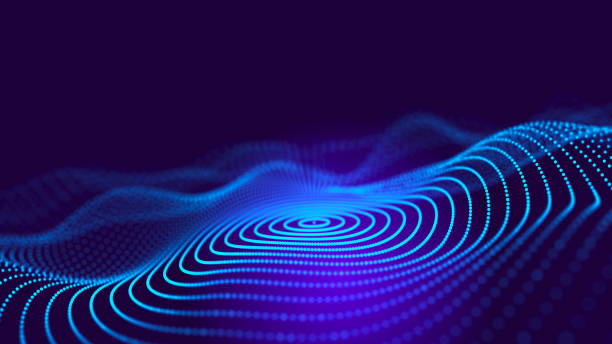
\includegraphics[scale=2.5]{img/page_de_garde.png} \\[1cm]
        \HRule \\[0.4cm]
        { \huge \bfseries LMECA2300 Advanced Numerical Methods \\[0.4cm] }
    
        \HRule \\[1.5cm]
        \textsc{\LARGE Simon Desmidt}\\[1cm]
        \vfill
        \vspace{2cm}
        {\large Academic year 2024-2025 - Q2}
        \vspace{0.4cm}
         
        
\includegraphics[width=0.15\textwidth]{img/epl.png}
        
        UCLouvain\\
    
    \end{center}
    \end{sffamily}
\end{titlepage}

\setcounter{tocdepth}{1}
\tableofcontents
\chapter{2-D acoustic and electromagnetic waves}
\section{Physical laws}
The expression of the force of the source applied to its surrounding is derived from Newton's law $F=ma$:
\begin{equation}
  \rho_0 \frac{\partial \vec{u}}{\partial t} + \nabla p = r_v
\end{equation}
where $\rho_0$ is the average density of the surrounding, $\vec{u}$ is the velocity field, $p$ is the variation of pressure and $r_v$ is the "pressure force". \\
The conservation law of energy is 
\begin{equation}
  \nabla \cdot \vec{u} + \chi \frac{\partial p}{\partial t}=s_v
\end{equation}
where $\chi$ is the compressibility $[kg^{-1}ms^2]$ and is given by the equation $\frac{\rho}{\rho_0}=\chi p$. $s_v$ is the "velocity source".\\
\section{Wave equation}
The wave equation is
\begin{equation}
	\nabla^2p-\rho_0\chi \frac{\partial^2 p}{\partial t^2} - -\rho_0 \frac{\partial s_V}{\partial t}
\end{equation}
In 1D, with $s_V=0$, the solution is any function $f\left(t-\frac{x}{v}\right)$ or $g\left(x-tv\right)$ with $v=1/\sqrt{\rho_0\chi}$. 
\section{Plane wave}
In the plane, the standard wave is given by 
\begin{equation}
	p(x,t)=p_0 \cos(\omega t-kx)
\end{equation}
where the phase velocity is $v_{ph} = \frac{\omega}{k}=\frac{1}{\sqrt{\chi \rho_0}}$.\\
The wave impedance is $\eta = \frac{p}{u_x} = \sqrt{\frac{\rho_0}{\chi}} \ [kgm^{-2}s^{-1}]$.
\section{Harmonic case}
In the case of a harmonic soundwave, we can use phasors:
\begin{equation}
  p(\vec r, t)=Re\{P(\vec r)e^{j\omega_0t}\}
\end{equation}
\begin{itemize}
  \item [$\to$] Note: there is a relationship between the phasors and the Fourier transform:
\end{itemize}
\begin{equation}
  F\{p\} = Re(P)\pi[\delta (\omega-\omega_0) + \delta (\omega+\omega_0)] + jIm(P)\pi[\delta (\omega-\omega_0) - \delta (\omega+\omega_0)]
\end{equation}
with $\omega$ the frequency variable.\\
In the frequency domain, the PDE becomes
\begin{equation}\label{eq:wave}
  \nabla^2 P+k^2 P= -j\omega \rho_0 S_V = Q 
\end{equation}
where $k$ is the wavenumber $k=2\pi/\lambda$. This is useful to make the time dependence disappear. 
\subsection{Green function}
The Green function is the solution $G$ to the following Fourier PDE;
\begin{equation}
  \nabla^2 G+k^2G = \delta(x)\delta (y)
\end{equation}
The general solution is 
\begin{equation}
  G(\rho) = -\frac{j}{4}H_0^{(2)} -\frac{j}{4}(J_0(k\rho) - jY_0(k\rho))
\end{equation}
where $J_0$ and $Y_0$ are respectively the Bessel functions of order 1 and 2, and $\rho$ is the distance between the source and the observer.\\
The Bessel functions $J_n(x)$ are solutions of the equation
\begin{equation}
  x^2J_n''(x)+xJ_n'(x) + (x^2-n^2) J_n(x)=0
\end{equation}
and there exists an approximation of the Hankel function $H_0^{(2)}$ for $x\gg 1$:
\begin{equation}
  H_0^{(2)}(x) \approx \sqrt{\frac{2}{\pi x}} e^{j\pi/4}e^{-jx}
\end{equation}
\subsection{From velocity source to pressure}
The pressure due to a velocity source spread over infinitesimal segment $\Gamma'$:
\begin{equation}
  p(r) = G(\vec r-\vec r') (j\omega \rho_0) v_n(\vec r')d\Gamma'
\end{equation}
To get the total pressure, we have to do an integral:
\begin{equation}
  p = p_{inc} + \frac{\omega \rho_0}{4} \int_\Gamma H_0^{(2)}(k|r-r'|)v_n(\vec r')d\Gamma'  
\end{equation}
Which is obtained from the velocity source $-j\omega \rho_0S_v$ from equation \eqref{eq:wave}, and doing a convolution with the Green function. \\

This integral can be approximated with a pointwise approach:
\begin{equation}
  I\approx C\sum_i v_iG(\rho_i)dl_i
\end{equation}
where $C=-j\omega\rho_0$, $v_i$ is the normal component of the velocity vector, and $dl_i$ the length of the segment.  
\end{document}